\documentclass[aspectratio=1610]{beamer}

\usetheme{unnslides}
\usefonttheme{professionalfonts}

\usepackage{listings}
\usepackage{graphicx}
\usepackage{caption}
\usepackage{cmbright}
\usepackage{fontspec}
\usepackage{unicode-math}
\usepackage{amsfonts}

\setromanfont{CMU Serif}
\setsansfont{CMU Sans Serif}
\setmathfont{Latin Modern Math}

\usepackage{polyglossia}
\setmainlanguage{russian}
%\setbeamertemplate{itemize item}{\color{black}$\blacktriangleright$}

\DeclareMathOperator*{\argmax}{arg\,max}
\DeclareMathOperator*{\argmin}{arg\,min}
\DeclareMathOperator{\sign}{sign}
\DeclareMathOperator{\re}{Re}

\graphicspath{ {../paper/images/}{img/} }
%set pages numeration
\setbeamertemplate{footline}[frame number]
\setbeamertemplate{headline}{}
\setlength\abovecaptionskip{-1pt}

\title{Исследование схем ускорения сходимости алгоритмов глобальной оптимизации}
\author{\textbf{Владислав~Соврасов}}
\institute{ННГУ им. Н.И. Лобачевского}
\date{}

\begin{document}

\begin{frame}[noframenumbering,plain]
\titlepage
\end{frame}

\begin{frame}
  \frametitle{Постановка задачи}
    \(D=\{y\in \mathbf{R}^N:a_i\leqslant x_i\leqslant{b_i}, 1\leqslant{i}\leqslant{N}\}\) ---
    некоторый гиперинтервал, на котором определены функции задачи.
  \begin{displaymath}
    \begin{array}{c}
      Q=\{y\in D: g_j(y)\leqslant 0,  1\leqslant{j}\leqslant{m}\}  \\
      \varphi(y^*)=\min\{\varphi(y):y\in Q\}
    \end{array}
  \end{displaymath}
  Предполагается, что целевая функция \(\varphi(y)\) и ограничения \(g_j(y)\) удовлетворяет условию Липшица в области \(D\):
  \begin{displaymath}
  |\varphi(y_1)-\varphi(y_2)|\leqslant L\Vert y_1-y_2\Vert,y_1,y_2\in D,0<L<\infty
  \end{displaymath}
  Численное решение задачи означает построение оценки \(\widetilde{y}\), близкой по какой-либо
  норме к точке \(y^*\) на основе конечного числа значений целевой функции задачи,
  вычисленных в точках области \(D\).
\end{frame}

\begin{frame}
  \frametitle{Редукция размерности}
  %Основные подходы:
  %\begin{itemize}
    %\item<1->
     Использование развёрток:
    \(\lbrace y\in \mathbf{R}^N:-2^{-1}\leqslant y_i\leqslant 2^{-1},1\leqslant i\leqslant N\rbrace=\{y(x):0\leqslant x\leqslant 1\}\),
    \(\varphi(y(x^*))=\min\{\varphi(y(x)):x\in [0;1]\}\)
    %\item<2->
    %\item<3-> Блочная многошаговая схема:

    %\(u_1=(y_1,y_2,\dots,y_{N_1}),u_2=(y_{N_1+1},y_{N_1+2},\dots,y_{N_1+N_2}),\dots,u_M=(y_{N-N_M+1},y_{N-N_M+2},\dots,y_N)\)
    %\(\min\limits_{y\in D}\varphi(y)=\min\limits_{u_1\in D_1}\min\limits_{u_2\in D_2}\dots\min\limits_{u_M\in D_M}\varphi(y)\)
  %\end{itemize}
  \begin{columns}
    \begin{column}{0.5\textwidth}
      \begin{figure}[ht]
        \centerline{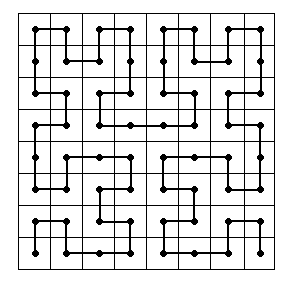
\includegraphics[width=.5\textwidth]{peano2d.png}}
      \end{figure}
    \end{column}
    \begin{column}{0.5\textwidth}
      \begin{figure}[ht]
      \centerline{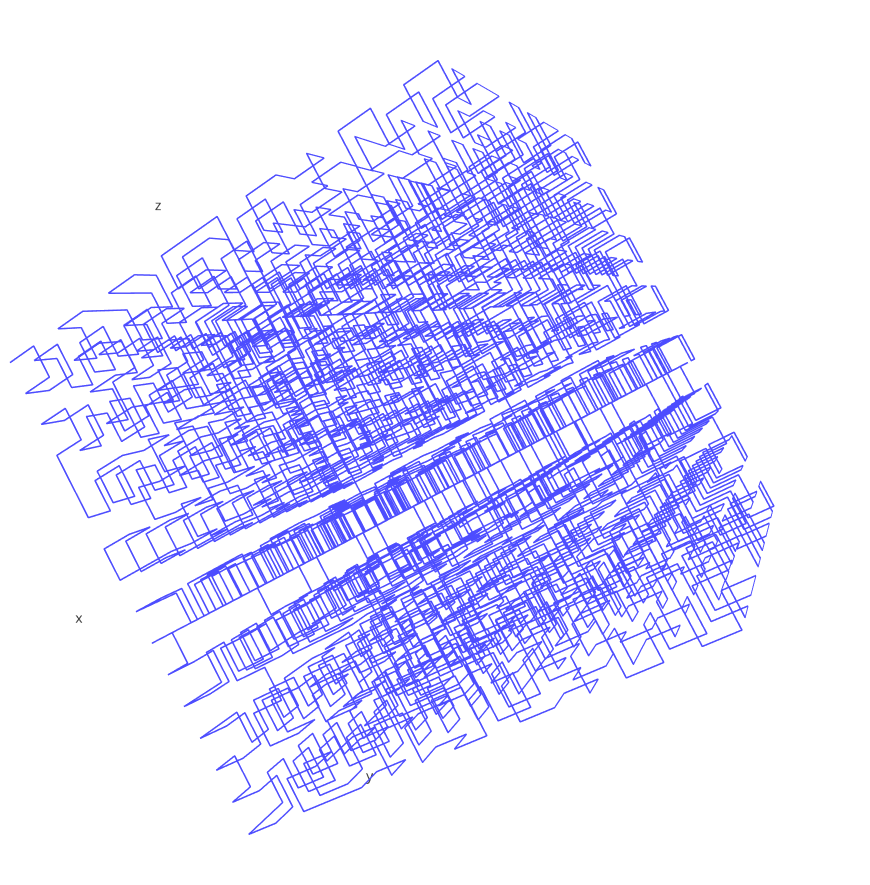
\includegraphics[width=.6\textwidth]{peano3d.png}}
      \end{figure}
    \end{column}
  \end{columns}
  Многошаговая схема:
  \(\min\limits_{(x_1,..,x_n)\in D} f(x_1,..,x_n)=\min\limits_{a_1\leqslant x_1\leqslant b_1}\min\limits_{a_2\leqslant x_2\leqslant b_2}...\min\limits_{a_n\leqslant x_n\leqslant b_n} f(x_1,...,x_n)\)
\end{frame}

\begin{frame}
  \frametitle{Метод глобальной оптимизации}
  Общая схема характеристического метода:
  пусть имеется \(k\) результатов испытаний, далее:
  \begin{enumerate}
    \setlength{\itemindent}{.1in}
    \item[Шаг 1.] Упорядочить поисковую информацию по возрастанию
    координат точек испытаний
    \item[Шаг 2.] Вычислить для каждого интервала
    величину \(R(i)\), называемую характеристикой.
    \item[Шаг 3.] Выбрать интервал номер \(t\) с наибольшей
    характеристикой и провести в нем испытание:
    \begin{displaymath}
      x^{k+1}=d(t)\in (x_{t-1}, x_t)
    \end{displaymath}
  \end{enumerate}

  Критерий остановки:
  \begin{displaymath}
    x_t - x_{t-1} < \varepsilon
  \end{displaymath}
\end{frame}

\begin{frame}
  \frametitle{Класс тестовых задач}
  \begin{columns}
    \begin{column}{0.5\textwidth}
      Генератор GKLS:
      \begin{displaymath}
        \begin{matrix}
          f(x)=
          \left\{
          \begin{matrix}
          C_i(x), x \in S_i, i\in 2,\dots ,m \\
          \Vert x-T \Vert^2 + t, x\not\in S_2,\dots,S_m
          \end{matrix} \right.
        \end{matrix}
      \end{displaymath}

      \begin{itemize}
        \item варьируемое число локальных минимумов;
        \item варьируемый размер области притяжения глобального минимума;
        \item размерность функции также задаётся.
      \end{itemize}
    \end{column}
    \begin{column}{0.5\textwidth}
      \centerline{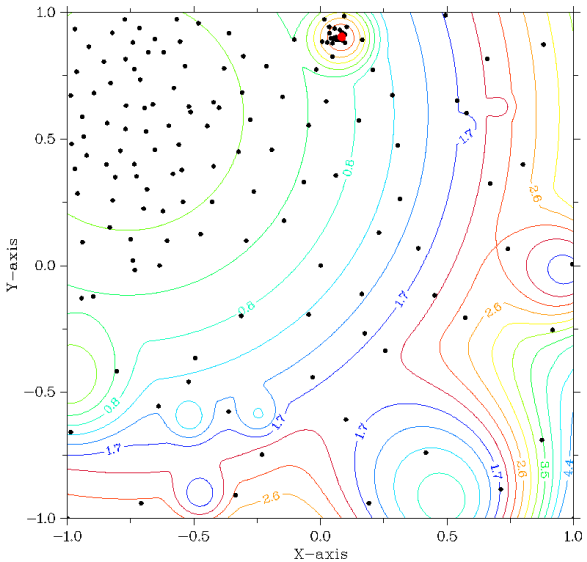
\includegraphics[width=0.9\textwidth]{gkls_color.png}}
    \end{column}
  \end{columns}
\end{frame}

\begin{frame}
\frametitle{Использование методов локальной оптимизации}
Способы использования локального поиска (метод Хука-Дживса):\
\begin{enumerate}
  \item Запуск из лучшей найденной точки после окончания работы АГП;
  \item Запуски из текущих лучших точек в процессе работы АГП.
\end{enumerate}
\bigbreak
Стратегии сохранения информации (для п. 2):
\begin{itemize}
  \item добавлять только лучшие точки;
  \item добавлять в поисковую информацию все точки.
\end{itemize}
\end{frame}

\begin{frame}
  \frametitle{Использование методов локальной оптимизации}
  Результаты применения различных стратегий сохранения информации:
  \begin{figure}[ht]
        \begin{minipage}[b]{0.49\linewidth}
            \centering
            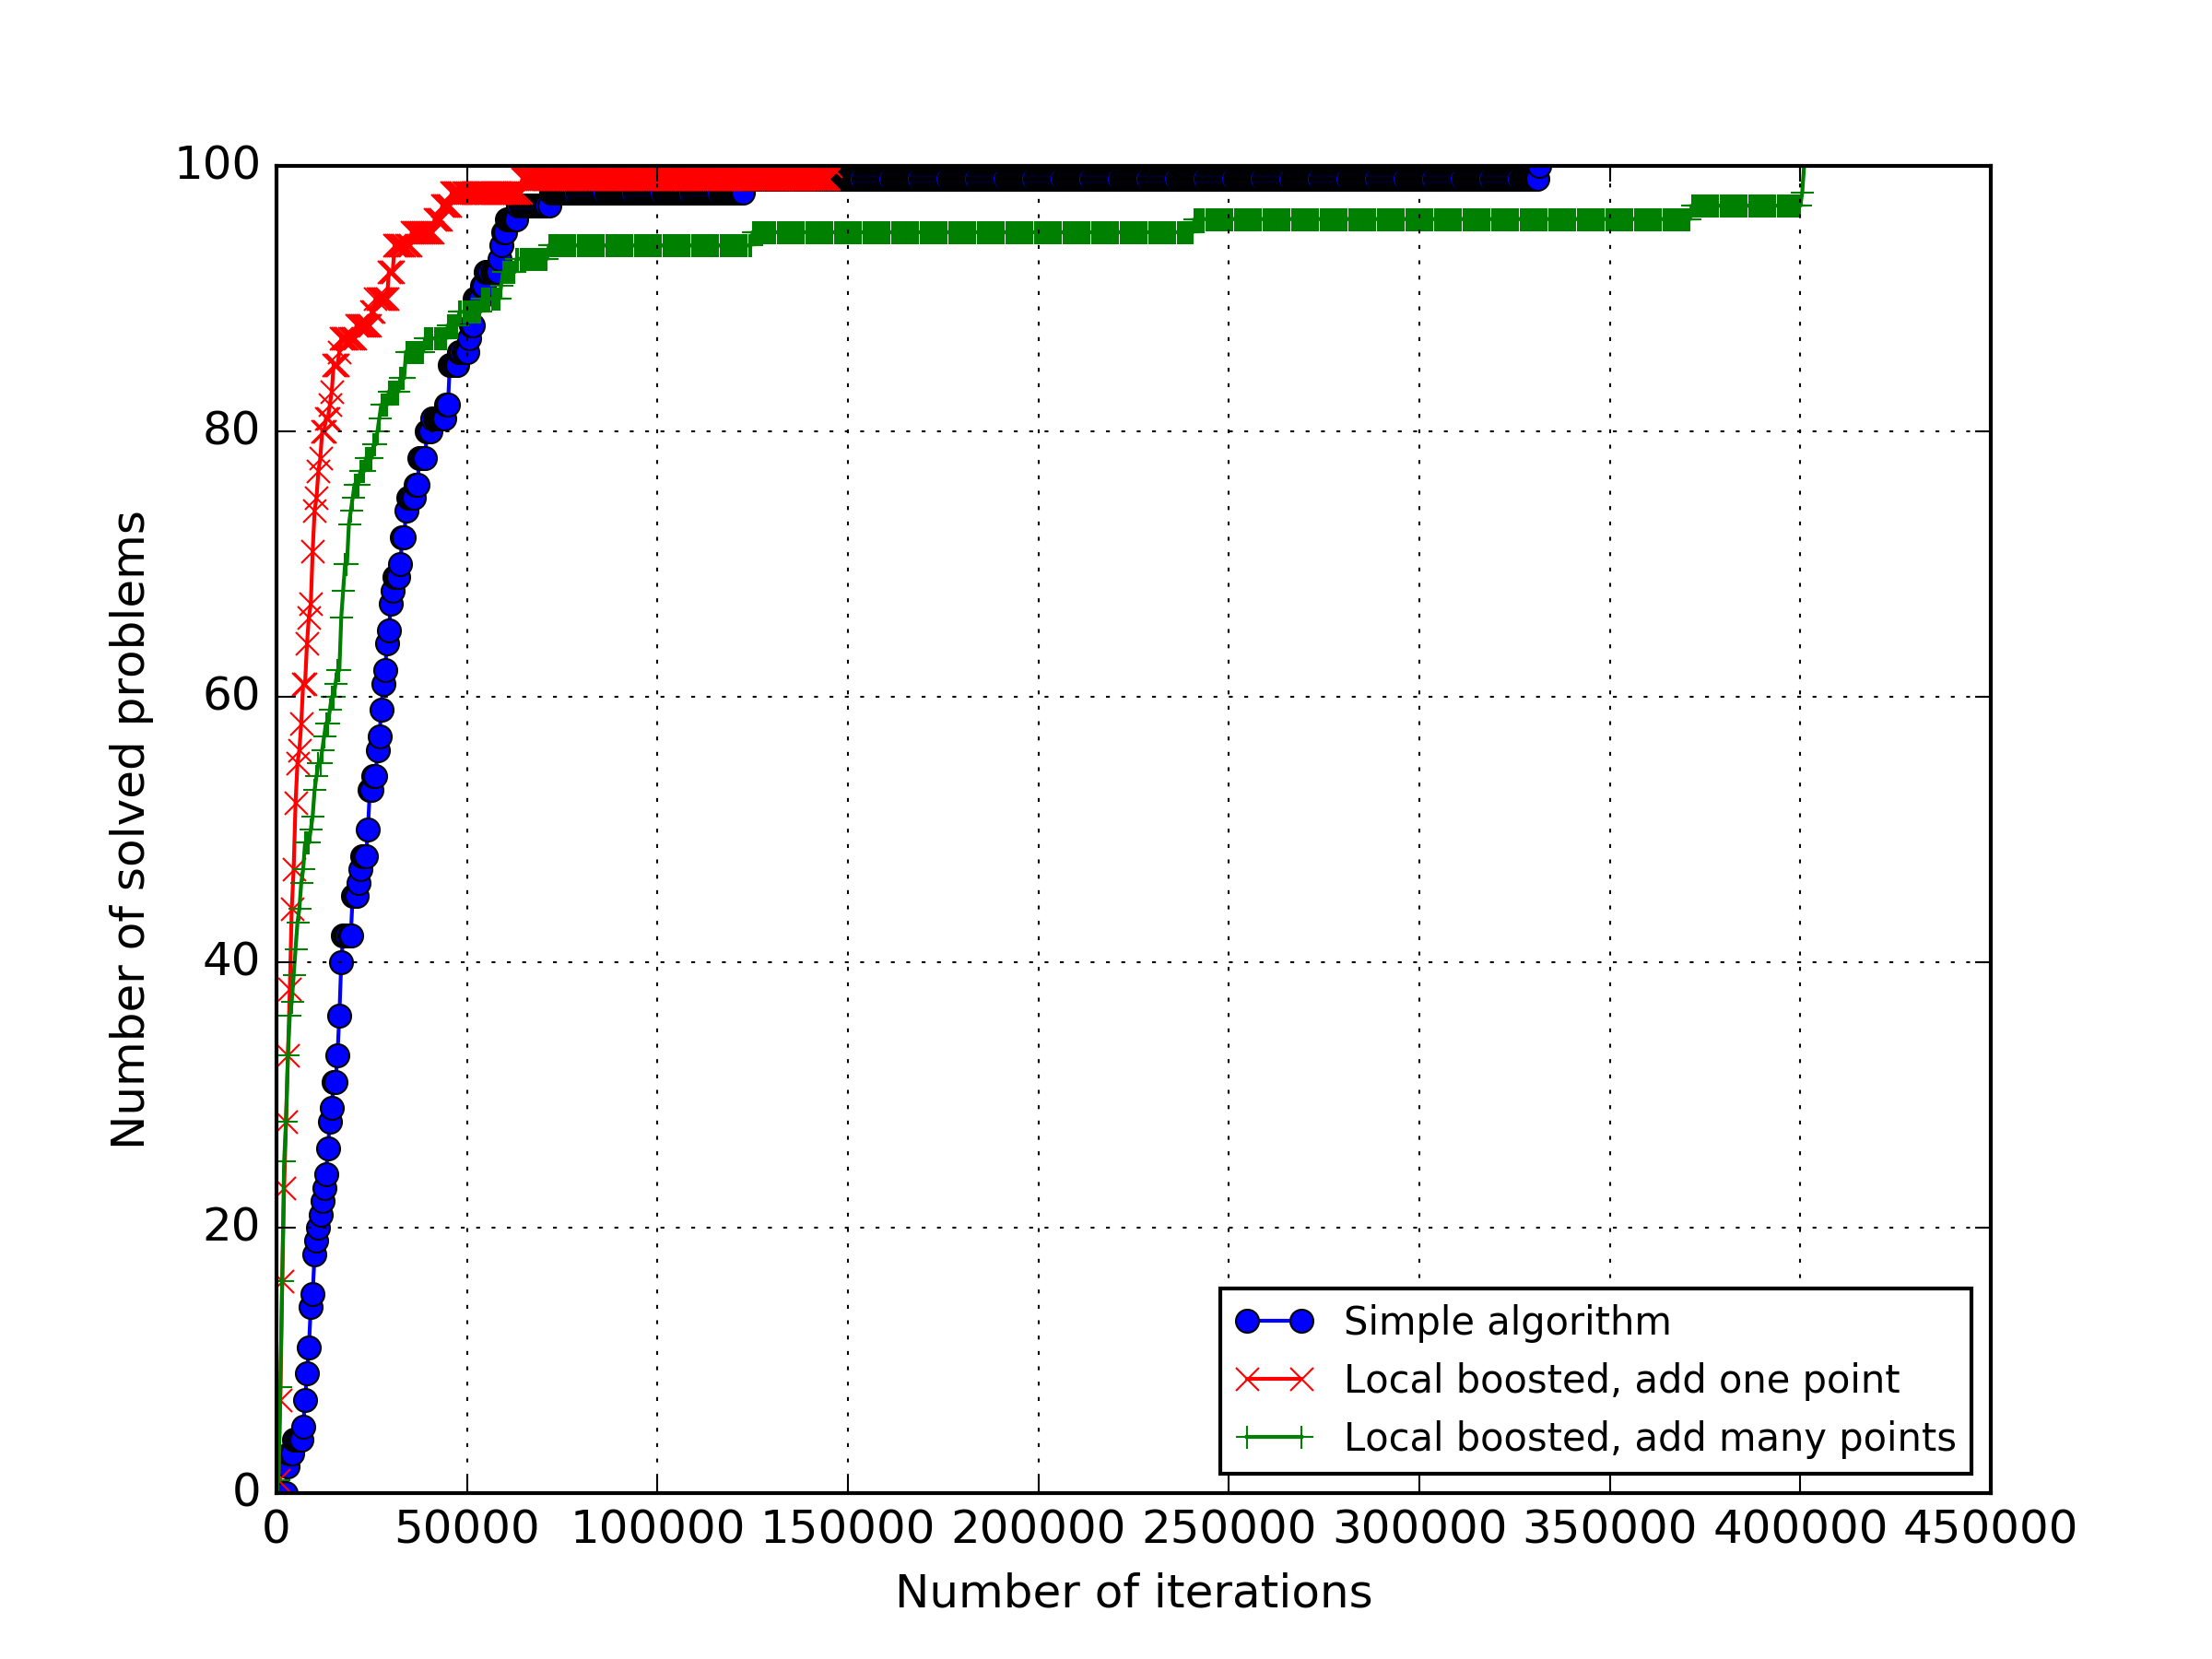
\includegraphics[width=\textwidth]{local_search_op.png}
            \caption*{GKLS 4d Simple}
        \end{minipage}
        \begin{minipage}[b]{0.49\linewidth}
            \centering
            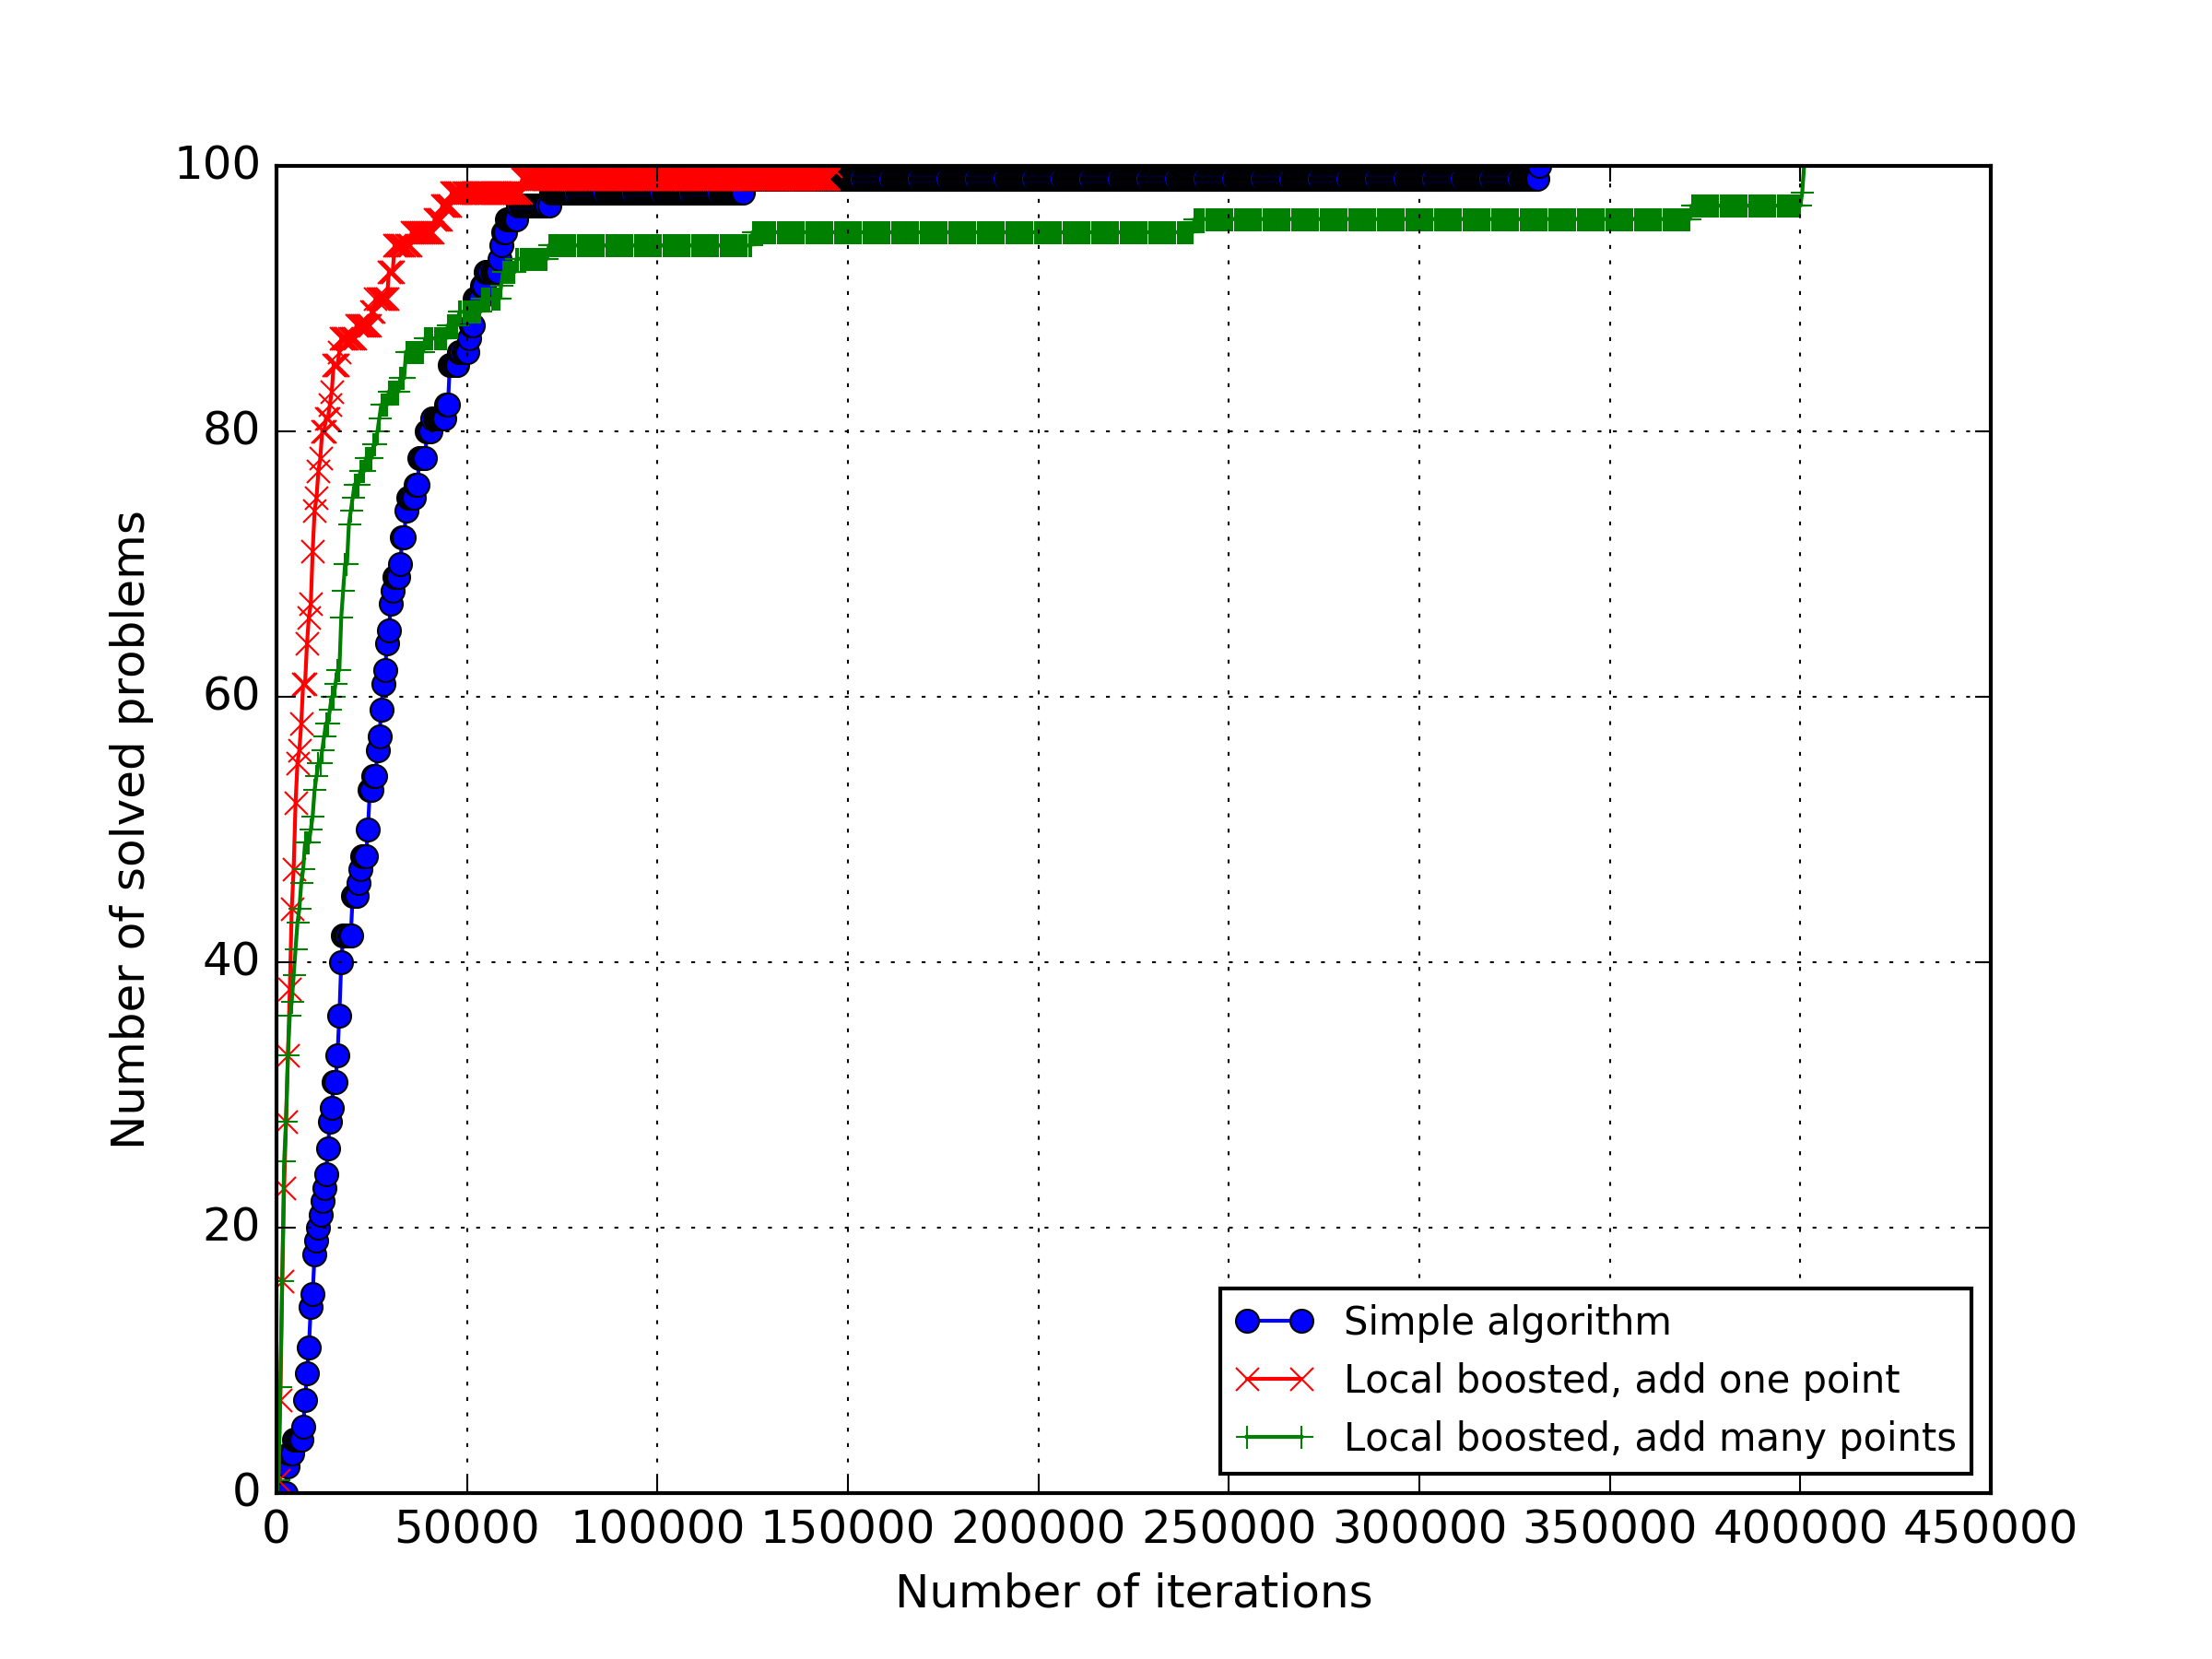
\includegraphics[width=\textwidth]{local_search_op.png}
            \caption*{GKLS 5d Simple}
        \end{minipage}
    \end{figure}
\end{frame}

\begin{frame}
\frametitle{Смешанный алгоритм}
Метод является модификацией АГП. Каждый интервал имеет две
характеристики \(R(i)\) и \(R^*(i)\).
  \begin{displaymath}
  R^*(i)=\frac{R(i)}{\sqrt{(z_i-z^*)(z_{i-1}-z^*)}/\mu + 1.5^{-\alpha}}
  \end{displaymath}
  Для эффективной реализации АГП используется приоритетная
  очередь интрервалов. Ключ – \(R(i)\).
  Для смешанного АГП – две связанные очереди.
  Операции с очередями:
  \begin{itemize}
    \item Синхронная вставка
    \item Синхронное удаление
    \item Обновление перекрестных ссылок при восстановлении кучеобразности
  \end{itemize}
\end{frame}

\begin{frame}
  \frametitle{Смешанный алгоритм}
  \begin{figure}
    \center
      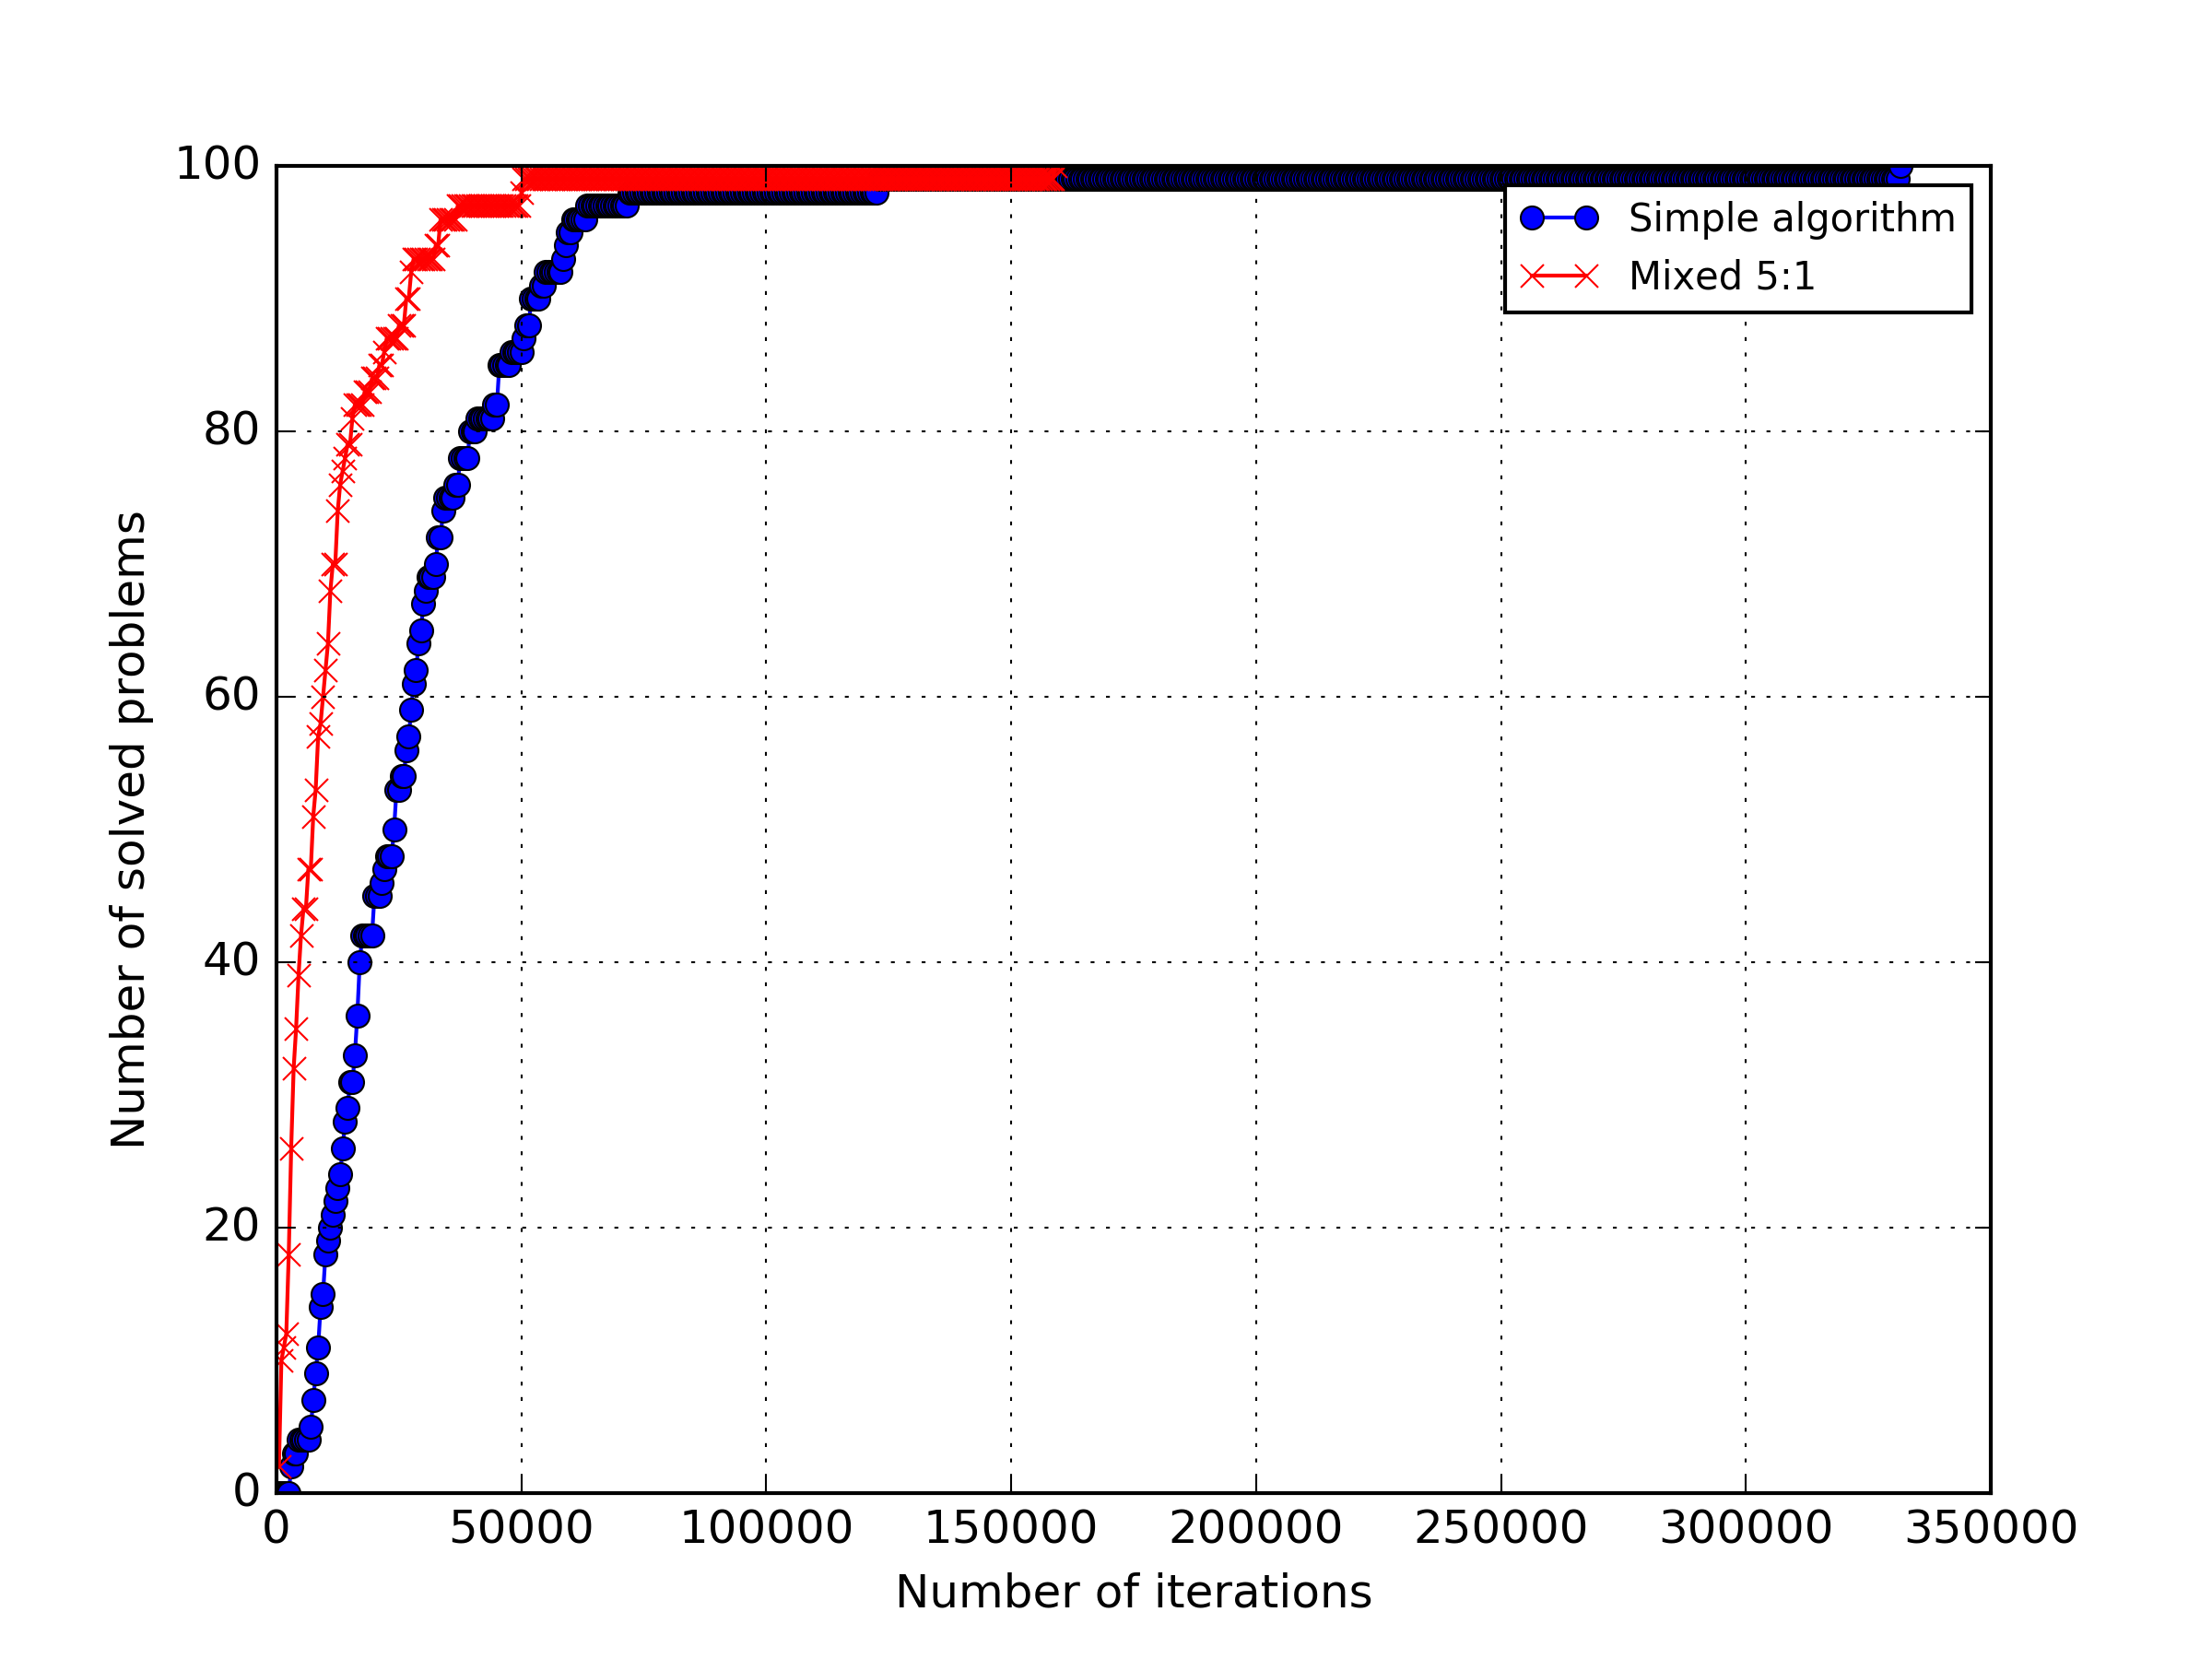
\includegraphics[width=0.7\textwidth]{mixed_op4d.png}
      \caption*{Операционные характеристики обычного и смешанного АГП на классе GKLS 4d Simple}
  \end{figure}
\end{frame}

%\begin{frame}
%\frametitle{Адаптивная оценка константы Гёльдера}
%  Вместо общей оценки \(M\) для каждого интервала вычисляется своя оценка \(M_i\):
%  \begin{displaymath}
%    \begin{array}{c}
%      H_i=\frac{|z_i-z_{i-1}|}{\Delta_i} \\
%      \lambda_i=\max\{H_{i-1},H_i,H_{i+1}\} \\
%      H^k=\max\{H_i:i=2,\dots ,k\} \\
%      \gamma_i=H^k\frac{\Delta_i}{\Delta^{max}} \\
%      \Delta^{max}=\max\{\Delta_{i}:i=2,\dots ,k\}
%    \end{array}
%  \end{displaymath}
%
%  \begin{displaymath}
%    M_i=r\cdot \max\{H_i, \frac{1}{2}(\lambda_i+\gamma_i),\xi\}
%  \end{displaymath}
%
%  \begin{displaymath}
%    \overline{M_i}=r\cdot \max\{H_i, \frac{\lambda_i}{r}+\frac{r-1}{r}\gamma_i,\xi\}
%  \end{displaymath}
%\end{frame}
%
%\begin{frame}
%\frametitle{Адаптивная оценка константы Гёльдера}
%\begin{columns}
%  \begin{column}{0.5\textwidth}
%    \begin{figure}[ht]
%      \centerline{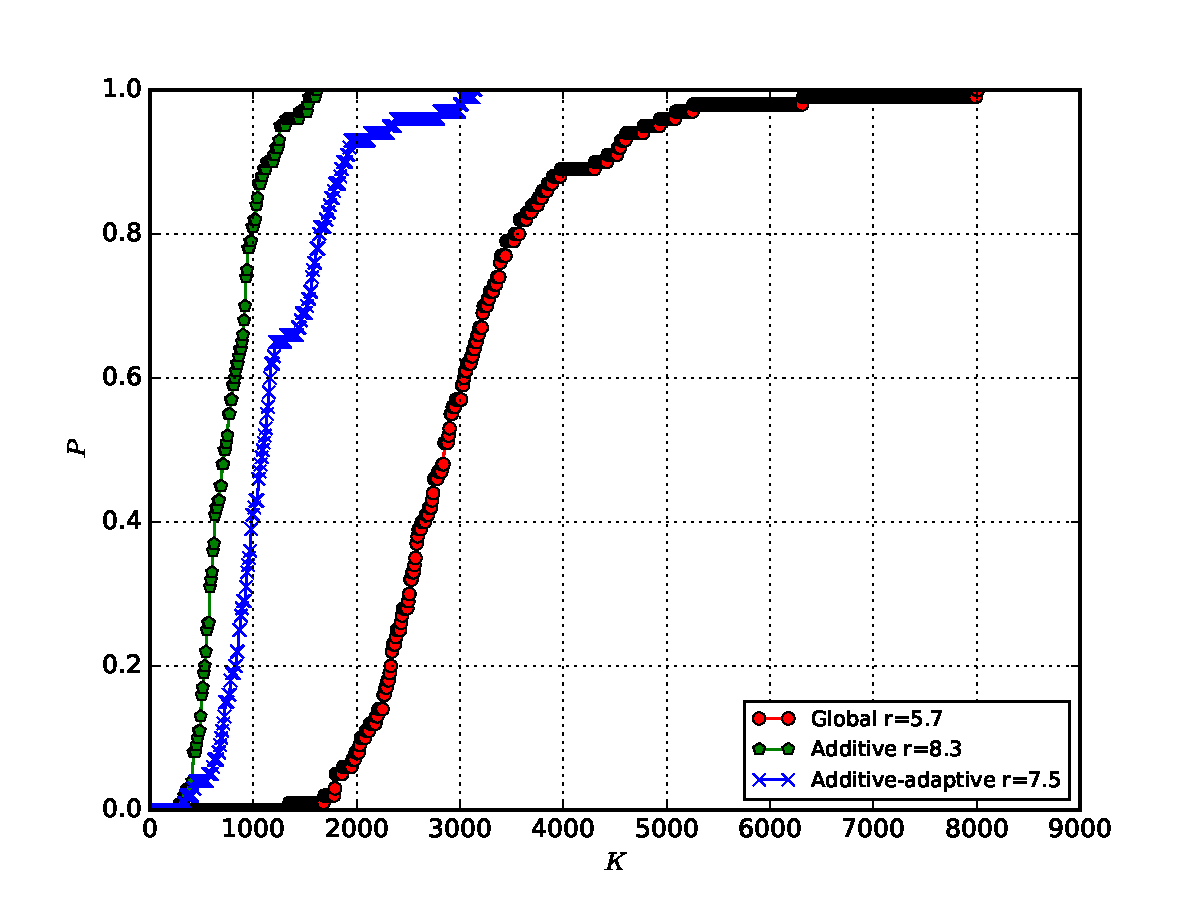
\includegraphics[width=1.1\textwidth]{gkls-s.pdf}}
%    \caption*{GKLS Simple 2d}
%    \end{figure}
%  \end{column}
%  \begin{column}{0.5\textwidth}
%    \begin{figure}[ht]
%    \centerline{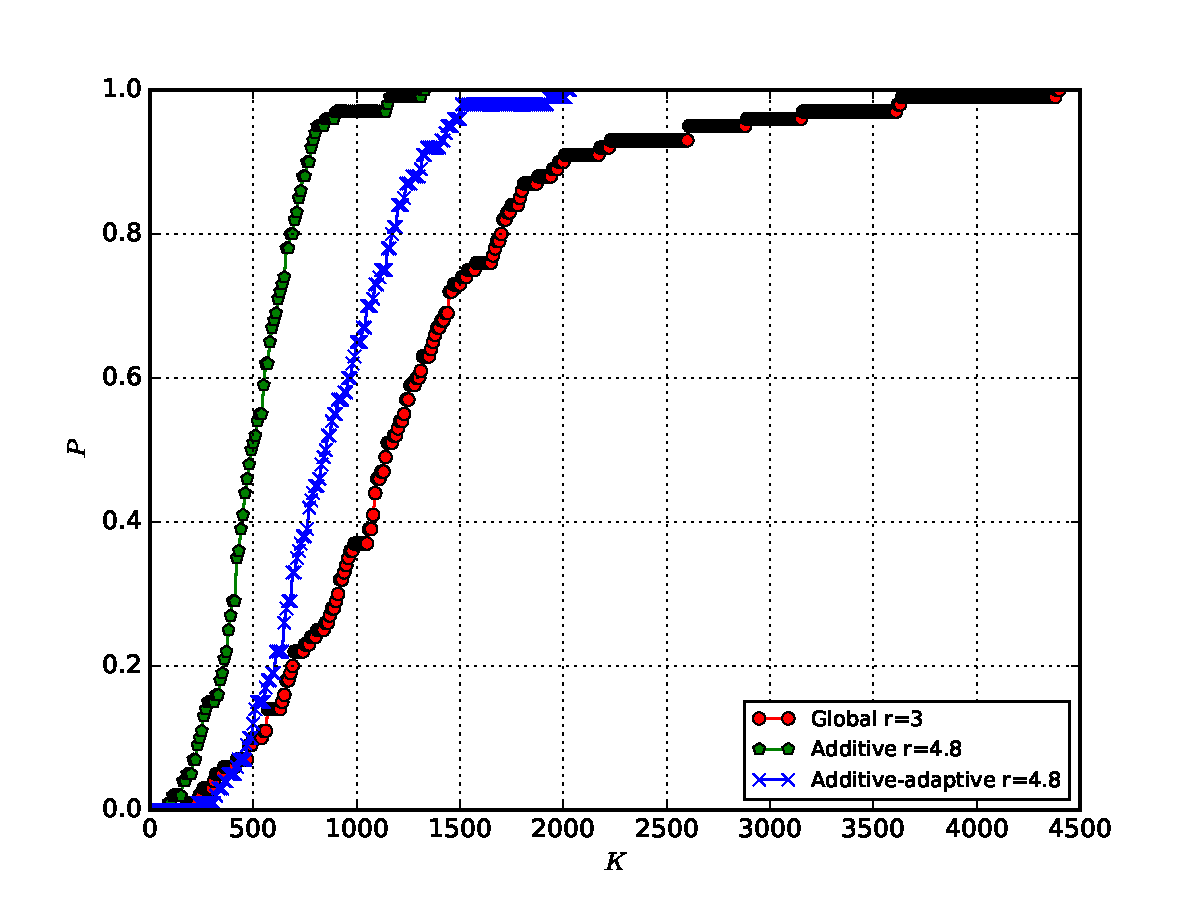
\includegraphics[width=1.1\textwidth]{grishagin.pdf}}
%    \caption*{\(F_{GR}\)}
%    \end{figure}
%  \end{column}
%\end{columns}
%
%\end{frame}

\begin{frame}
  \frametitle{Пример прикладной задачи}
  \begin{columns}
    \begin{column}{0.7\textwidth}

      Рассматривется система из \(n\) материальных точек, связанных упруго-диссипативными элементами.
      Например, при \(n=2\):
      \begin{displaymath}
        \begin{array}{cr}
          \begin{cases}
            \ddot \xi_1 = -\beta(\dot\xi_1 - \dot\xi_2) - \xi_1 + \xi_2 + u + v \\
            \ddot \xi_2 = -\beta(\dot\xi_2 - \dot\xi_1) - \xi_2 + \xi_1 + v
          \end{cases} \\
          \xi_1(0)=\xi_2(0),\;\dot\xi_1(0)=\dot\xi_2(0)=0
      \end{array}
      \end{displaymath}

      В реальной задаче \(n=10\), состояние не полностью наблюдаемо.

    \end{column}
    \begin{column}{0.3\textwidth}
      \centerline{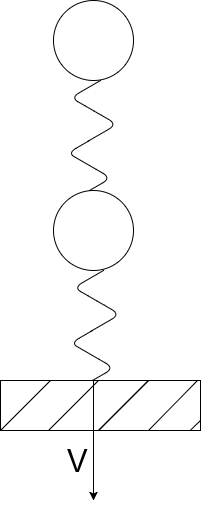
\includegraphics[width=.5\textwidth]{spring.png}}
    \end{column}
  \end{columns}

\end{frame}

\begin{frame}
  \frametitle{Пример прикладной задачи (результаты)}
  \begin{columns}
    \begin{column}{0.4\textwidth}

      Постановка задачи в методе главного критерия:
      \begin{align*}
        J_2(\Theta^*)=\min\{J_2(\Theta): J_1(\Theta) < \varepsilon, \\
        g_0(\Theta)\leqslant 0\}
      \end{align*}

      Решается серия задач трёхмерных при различных значениях \(\varepsilon\). Глобально-оптимальное решение
      при каждом \(\varepsilon\) --- Слейтерова точка в исходной задаче.

    \end{column}
    \begin{column}{0.5\textwidth}
      \centerline{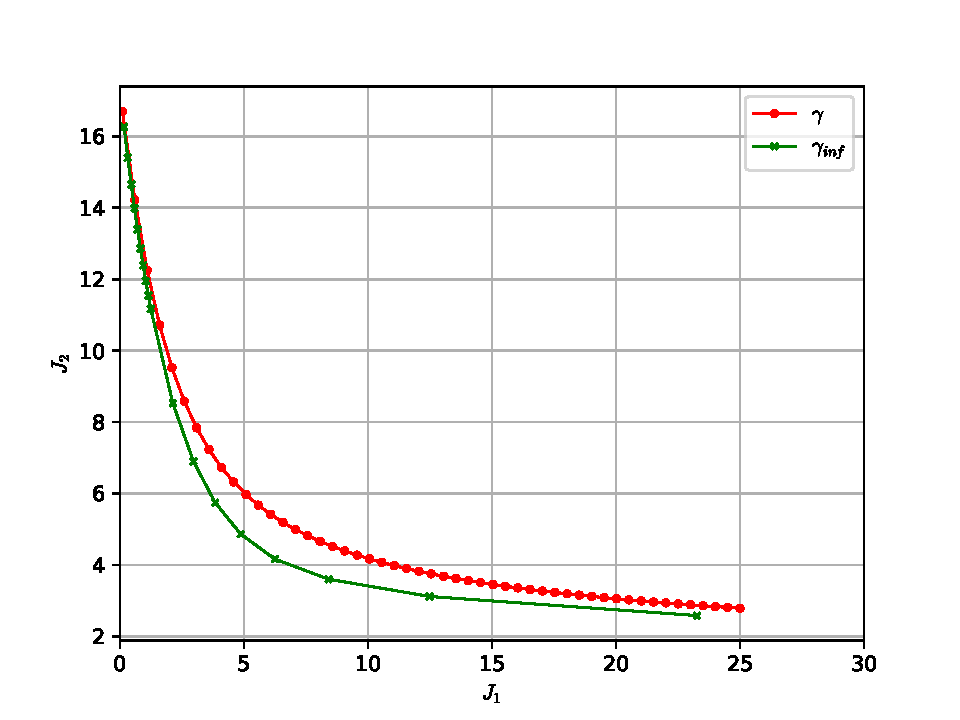
\includegraphics[width=1.2\textwidth]{solution.pdf}}
    \end{column}
  \end{columns}

\end{frame}

\begin{frame}{{}}
  \frametitle{ }
  \begin{center}
    \Large{Спасибо за внимание!}

\vspace{1cm}
    Владислав Соврасов

    sovrasov.vlad@gmail.com
  \end{center}
\end{frame}

\end{document}
